\chapter{Literature Review}\label{chap:Literature Review}
\section{Background}
Throughout the history of computer programming, most programming languages have been based on the English Language. However, the first-ever high-level programming language, "Plankalkül," designed by German Civil Engineer Konrad Zuse, was based on the German language \cite{arawjo2020write}. This programming language was designed mainly to replace Assembly language because it was noticed that it requires a great amount of mental effort. One of the advantages of high-level programming languages was that short code statements represented mathematical expressions in an understandable and readable form. Finally, the program written using high-level programming language had to be interpreted to machine code every time it ran, making the process match slower than running the equivalent machine code directly.

Different approaches to programming have evolved gradually. The programming paradigm concept began to rise. The first paradigm was the lowest-level programming paradigm, which was machine code that represented instructions in binary format. The next paradigm developed was the procedural paradigm. These languages (high-level languages) use vocabulary related to the problem being solved, and they describe exactly the procedure that should be followed to solve a specific problem. Then the \ac{OOP} languages were created, and in these languages, data and methods to manipulate it are kept as one entity called an object. In OOP, the only way to access the data is through the object's methods, guaranteeing flawless encapsulation. Then there were further programming paradigms, including imperative programming, declarative programming, functional programming, logic programming, and symbolic programming. Imperative programming is structured as a human-centered web, while declarative programming languages tell the computer what the problem is instead of telling how to solve it. Functional programming uses functions and recursion rather than assigning variables, while logic programming views computation as automated reasoning. Symbolic programming allows programs to manipulate formulas and program components as data. Finally, differentiable programming structures programs so they can be differentiated throughout \cite{programmingparadigms}.

Many attempts were made to design and implement localized programming languages. In order to design a localized language or understand how it is designed, I must first understand the tools and components needed to build a programming language.

A scanner (or lexer) takes the source code as a stream of characters and assembles them into individual tokens. These tokens can be single characters like ( and, or multi-character sequences like numbers (123), string literals ("hi!"), and identifiers (min).
Certain characters in a source file are not important. Whitespace is usually irrelevant (with Python being one of the notable exceptions), and comments are disregarded by the language by definition. The scanner typically discards these, leaving only meaningful tokens in a clean sequence \cite{nystrom2021crafting}. For example:
\begin{figure}[ht]
\centering
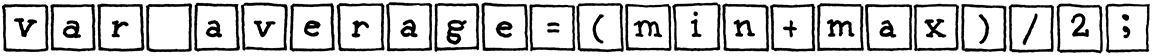
\includegraphics[width=15cm]{ch2-images/source-ccode.png}
\caption{Source Code \cite{nystrom2021crafting}}
\label{fig:Source Code}
\end{figure}

A lexer would turn the above code into the following set of tokens:
\begin{figure}[ht]
\centering
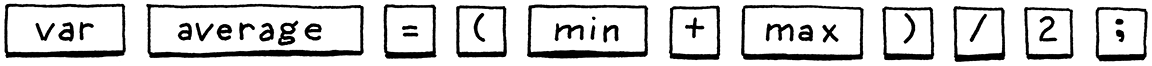
\includegraphics[width=15cm]{ch2-images/tokens.png}
\caption{Tokens \cite{nystrom2021crafting}}
\label{fig:Tokens}
\end{figure}

After scanning the source code, the next step for code processing is parsing. A parser takes the tokens generated by the lexer and constructs a parse tree (also called \ac{AST}) which reflects the language's grammar. For example, the above set of tokens is turned into the following tree:
\begin{figure}[ht]
\centering
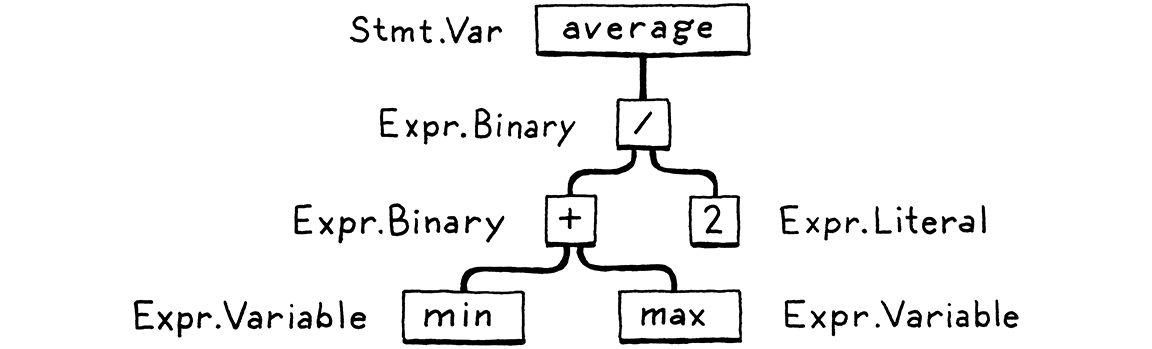
\includegraphics[width=15cm]{ch2-images/parser.png}
\caption{Syntax Tree \cite{nystrom2021crafting}}
\label{fig:Syntax Tree}
\end{figure}

It’s also the parser's job to detect code that violates the grammar rules of the language and report syntax errors.
Some language implementations have a tree-walk interpreter that traverses the AST to run the program. Other language implementations can use the syntax tree to transpile the program to a different high-level programming language \cite{nystrom2021crafting}.

After parsing the AST, the next step for code processing is the static analysis. A static analyzer uses the AST to perform binding and scope resolution, which determines what an identifier refers to. If the language is statically typed, type checking occurs at this stage, and type errors are reported if the language rules are violated.

The lexer, parser, and static analyzer are called the front end of the language implementation.

The last two steps are code optimization and code generation. Code optimization is replacing a line of code or a group of lines with a different code which is more efficient than the code written by the user as it uses less memory and runs faster. This step takes place just before generating the code. Finally, code generation takes place where a compiler generates the program's equivalent bytecode, which is then converted to machine code for a target processor architecture and operating system, or a transpiler which generates code in a target high-level programming language \cite{nystrom2021crafting}.

The code optimizer and the code generator are called the back end of the language implementation.

The following figure includes all parts of a programming language and summarizes the process of building a new programming language:
\begin{figure}[ht]
\centering
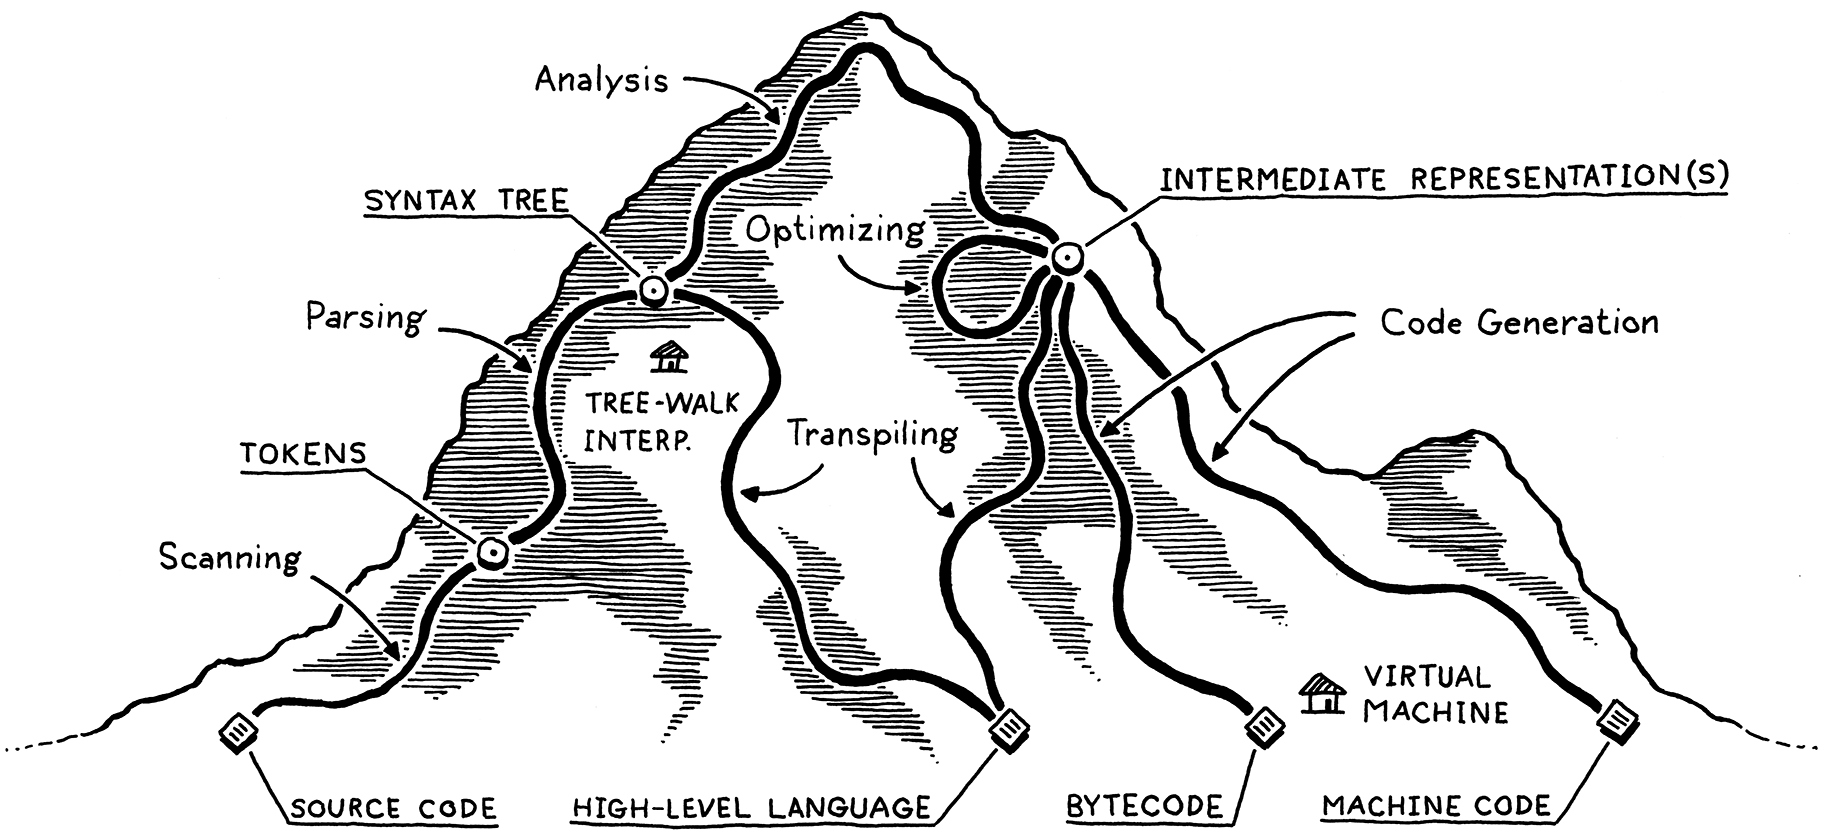
\includegraphics[width=15cm]{ch2-images/mountain.png}
\caption{Programming Language Mountain \cite{nystrom2021crafting}}
\label{fig:Programming Language Mountain}
\end{figure}

In order to use a programming language in writing a program, a code editor must be used. A code editor is an application used to edit source code. It typically includes features like syntax highlighting, code completion, and a debugger. An \ac{IDE} is an application that includes a code editor and other features like tools for unit testing, issue tracking, etc.

Eclipse is one of the most well-known IDEs for computer programming, with a base workspace and a customizable plugin system. Eclipse is mainly used for Java development but can also be used for other programming languages through plugins, such as C++, Python, PHP, and other languages. Eclipse is written mostly in Java, and its \ac{SDK}, which is a set of tools to build software for a particular platform, is free and open-source software released under the Eclipse Public License. Moreover, it allows users to write and contribute their own plugin modules \cite{eclipseide}.

Eclipse Plugins are computer programs that can be included with Eclipse to increase functionality and personalize the workspace. New features and functionalities, including support for additional programming languages, testing frameworks, and build systems, as well as new user interfaces and visualizations, can be offered via these plugins. Plugins can be downloaded and manually installed, or they can be installed and managed using the Eclipse Marketplace. Eclipse's extensible plugin design enables programmers to create and share their own plugins with the community \cite{eclipseplugins}.
\section{Previous Work for Programming Language Localization}
As mentioned before, many attempts were made to design a localized programming language in Arabic and other languages. In this section, I will discuss some of the previous work to localize a programming language or implement a non-English programming language.
\subsection{Babylscript}
 Iu \cite{iu2011babylscript} created Babylscript, which is a multilingual version of JavaScript. It allows programmers to write code using several languages and transition between language modes while doing so. By allowing several names to be attached to a single data item, Babylscript improves characteristics and makes it possible to create libraries with translated functions and object names for different languages. The following figure shows an example of Babylscript code:
\begin{figure}[ht]
\centering
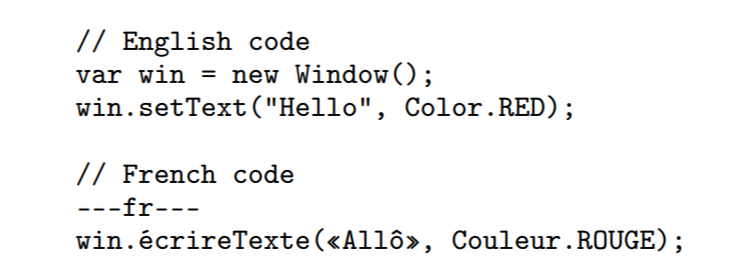
\includegraphics[width=10cm]{ch2-images/babylscript.png}
\caption{Babylscript Code \cite{iu2011babylscript}}
\label{fig:Babylscript Code}
\end{figure}

The architecture of Babylscript is based on the observation that punctuation and mathematical notations are shared by all natural languages. Therefore, it has a syntax that all languages share. Babylscript shares the same grammar for all language modes, despite the fact that various language modes may use different names for functions, objects, and methods as well as distinct tokens for keywords and operations. To switch between different language modes, programmers must write a command using three minus signs followed by the language they want to use followed by another three minus signs (see figure \ref{fig:Babylscript Code}). All keywords and symbols are translated into the new language as soon as the programmer switches the language mode. By enabling properties to have more than one translation in addition to their default name, Babylscript enhances the JavaScript object model. Therefore, if a translated name is available, programmers can access any property using that name instead of the default one. The following figure shows an example of property translation:

\begin{figure}[H]
\centering
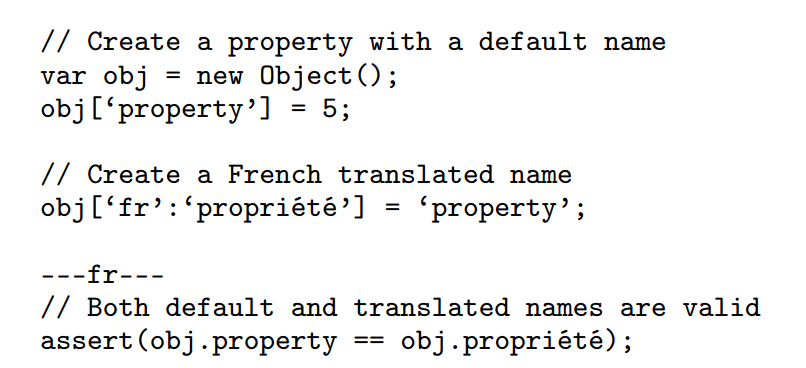
\includegraphics{ch2-images/babylscript2.png}
\caption{Babylscript Property Translation \cite{iu2011babylscript}}
\label{fig:Babylscript Property Translation}
\end{figure}

Babylscript is an extension of Mozilla Rhino JavaScript interpreter that uses the same parser, bytecode generator, and bytecode for all language modes because it uses the same grammar for all languages. However, each language has its own tokenizer to identify keywords and other tokens. Language context must be tracked by Babylscript's compiler because the access of properties of an object is dependent on the language mode. This is done by adding language tags to all structures passed between stages of the compiler. During tokenization, Babylscript's tokenizers convert keywords into a standard form, such as English, while leaving identifiers untouched. Since JavaScript names are resolved at runtime, the interpreter requires the language tags to detect the correct table of translated names for an object. The following figure shows how Babylscript is designed:
\begin{figure}[H]
\centering
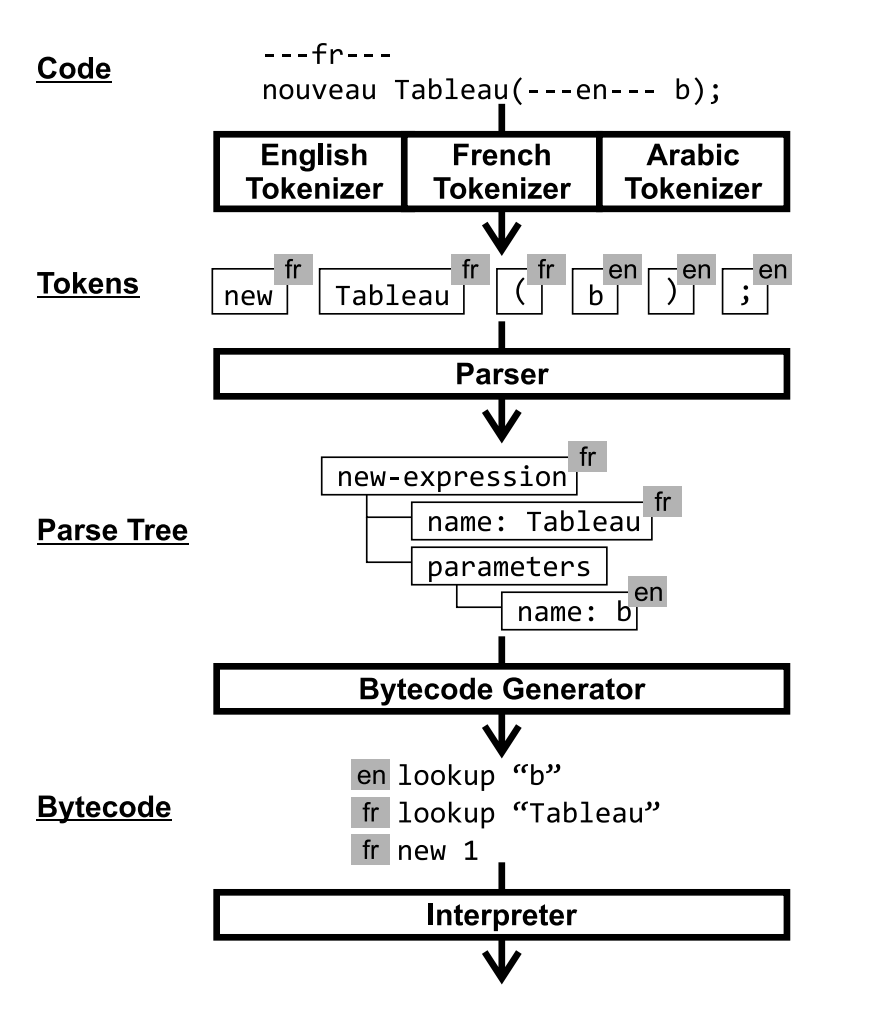
\includegraphics[width=7.3cm]{ch2-images/babylscript3.png}
\caption{Babylscript Implementation \cite{iu2011babylscript}}
\label{fig:Babylscript Implementation}
\end{figure}

Babylscript's language design allows programmers to write code using their own native language without being aware of Babylscript's support for other languages. In the future, some of the ideas behind Babylscript could be applied to statically typed languages like Java.
\subsection{Phoenix}
 Bassil \cite{bassil2019phoenix} created Phoenix, which is a computer programming language based on Arabic. It is a compiled, object-oriented, high-level, imperative, and general-purpose programming language. Phoenix is regarded as a C\# programming language localization. Both share the same syntax, and Phoenix uses features of modern languages to make Arabic programming easier. Phoenix is compiled from source code to machine code before being executed, just like C\#. Its current version runs on the Windows operating system and has the ability to convert compiled machine code into an executable file. Phoenix also comes with a suitable and user-friendly IDE that enables developers to write, save, debug, and compile their source code.

Phoenix is a modern programming language that offers many features that are suitable for computer programming. It includes supporting strong data types such as Decimal, String, Recursion, implicit type conversion between data types, conditional structures (if and if-else), and many other features.

The Phoenix compiler consists of six building blocks: preprocessor, scanner, parser, semantic analyzer, code generator, and linker. Each of these blocks will be discussed in detail.

The preprocessor helps in code simplification by eliminating extra information from the source code, including code comments and unneeded variables, and integrating third-party libraries. The scanner then tokenizes the simplified source code into understandable units known as tokens. The parser then examines the tokens created by the scanner to see if they comply with the programming language's syntax and grammar. The Phoenix parser is based on a \ac{CFG} as it provides powerful features including but not limited to recursion and nesting. The semantic analyzer then checks whether the code follows the semantics of the language, and then the parse tree is translated into executable code by the code generator. This code could be bytecode, machine code, or any other high-level programming language. Finally, the linker converts the target code into a stand-alone executable that can run on the operating system. 

The algorithm of the scanner is based on the \ac{FSM} to detect and tokenize identifier/variable names, numeric values, and string values, respectively. Phoenix keywords are also detected by the scanner. The following figures show the FSMs mentioned:

\begin{figure}[H]
\centering
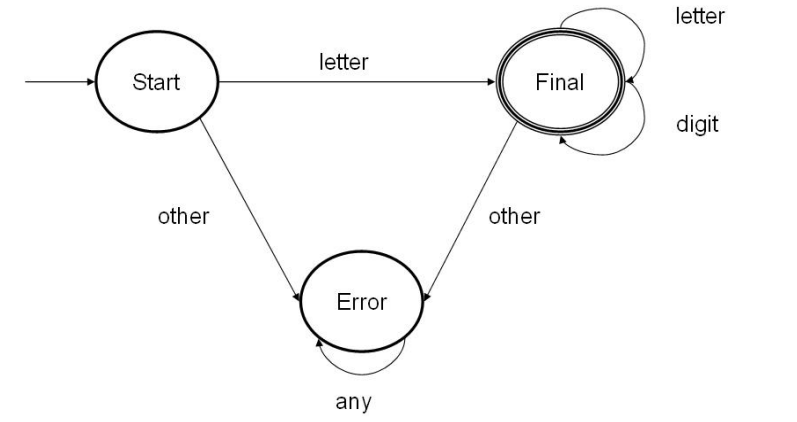
\includegraphics[width=10cm]{ch2-images/phoenix.png}
\caption{Finite Automata for Identifiers \cite{bassil2019phoenix}}
\label{fig:Finite Automata for Identifiers}
\end{figure}

\begin{figure}[H]
\centering
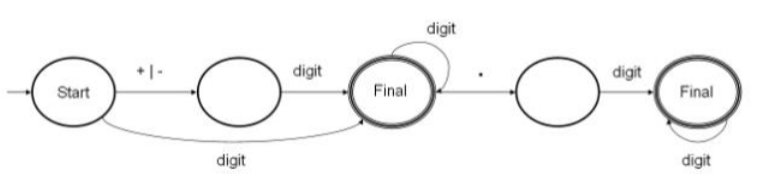
\includegraphics[width=10cm]{ch2-images/phoenix2.png}
\caption{Finite Automata for Numeric Values \cite{bassil2019phoenix}}
\label{fig:Finite Automata for Numeric Values}
\end{figure}

\begin{figure}[H]
\centering
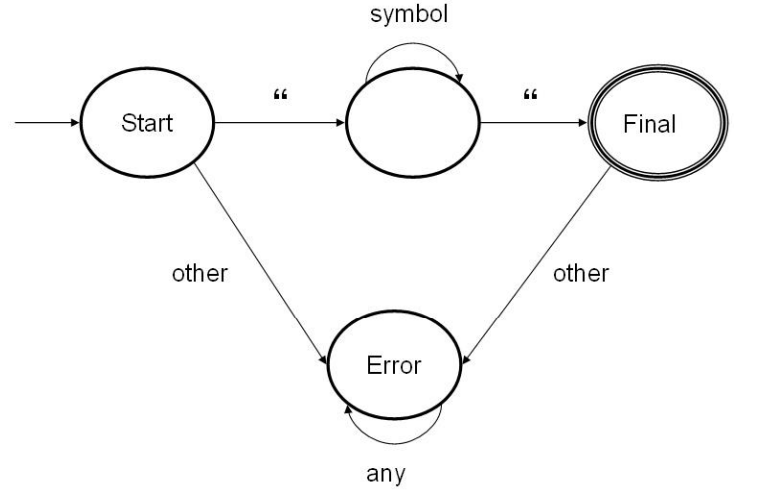
\includegraphics[width=10cm]{ch2-images/phoenix3.png}
\caption{Finite Automata for String Values \cite{bassil2019phoenix}}
\label{fig:Finite Automata for String Values}
\end{figure}

In the following figures, we will see a sample code written using Phoenix in an IDE designed especially for Phoenix and its equivalent C\# code:

\begin{figure}[H]
\centering
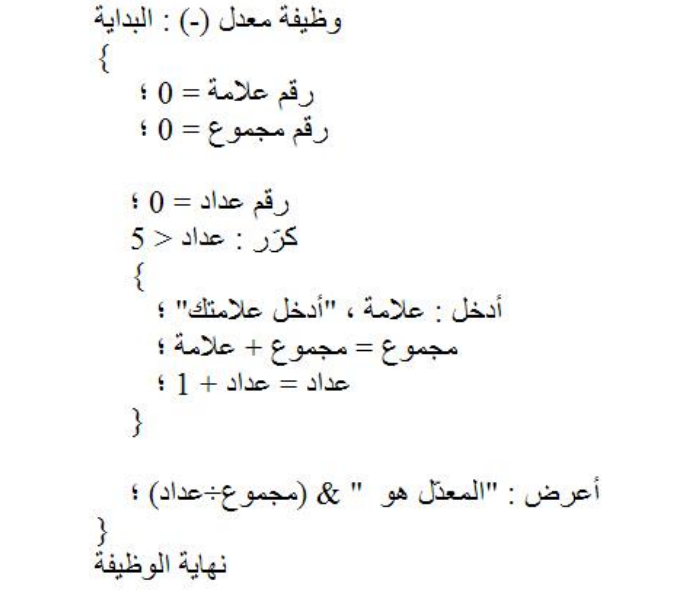
\includegraphics[width=8.5cm]{ch2-images/phoenix4.png}
\caption{Source code written using Phoenix \cite{bassil2019phoenix}}
\label{fig:Source code written using Phoenix}
\end{figure}

\begin{figure}[H]
\centering
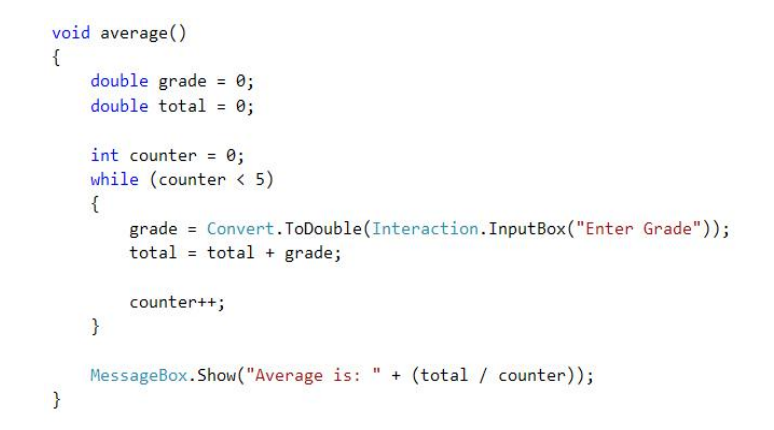
\includegraphics[width=15cm]{ch2-images/phoenix5.png}
\caption{Equivalent Source-Code written using C\# \cite{bassil2019phoenix}}
\label{fig:Equivalent Source-Code written using C\#}
\end{figure}

The results have shown several powerful features of Phoenix, including functions, while-loop, and arithmetic operations and its capability to build general-purpose programs that can be used for real-world applications. Phoenix might eventually get some additional object-oriented features, including inheritance, encapsulation, abstraction, and polymorphism. Additionally, a library of built-in classes and reusable functions is to be created with the aim of supplying several functionalities like file processing and database access.
\subsection{ARABLAN}
Al-A’ali and Hamid \cite{al1996design} created ARABLAN (or ARABLANG) which is another example of an Arabic programming language. It is a localization of Pascal programming language, and its mainly designed for non-English speaking school students to develop their computer programming skills. Learning ARABLAN is challenging for those whose native language is neither English nor Arabic. 

A few design decisions must be made while creating a programming language. In fact, various design decisions were made for ARABLAN, such as making it a high-level, sequential, imperative, and simple language to learn. The language uses relevant Arabic words that are simple to recall to make it simple to learn. Additionally, it achieves mobility and portability via the popular and affordable Arabic interface tool ``Nafitha." 

The syntax of the ARABLAN language is built with efficiency for both translation and execution. This is accomplished by adhering to certain rules, such as avoiding backtracking during parsing, ensuring an unambiguous grammar, avoiding dynamic storage allocation, using an appropriate internal form that can be executed directly, and reserving specific words for designated usages. 

The language allows the creation of two distinct types of declarations: constant declarations and variable declarations. An ARABLAN program begins with the declarations section, which is followed by the main program section, which contains the statements that can be executed. There are different types of statements, including assignment statements, selection statements, repetition statements, and input/output statements. Moreover, programmers can write subprograms in ARABLAN, which are parts of the main program. There are two different types of subprograms just like Pascal. 

The first two figures are two examples explaining the two types of declaration. The first figure is an example of the Constants Declaration, while the second figure is an example of the Variables Declaration:

\begin{figure}[h]
\centering
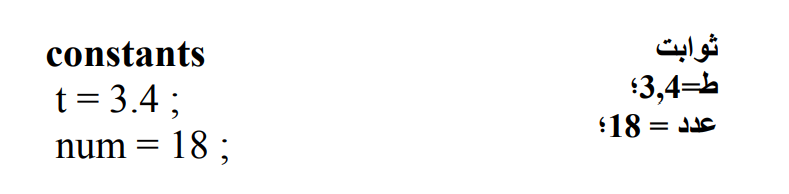
\includegraphics[width=8cm]{ch2-images/ARABLAN.png}
\caption{ARABLAN Constants Declaration \cite{al2007evaluation}}
\label{fig:ARABLAN Constants Declaration}
\end{figure}

\begin{figure}[h]
\centering
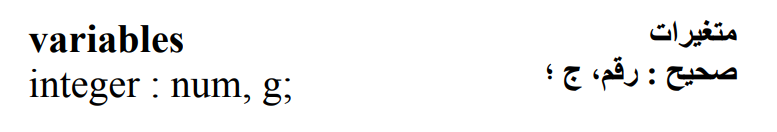
\includegraphics[width=8cm]{ch2-images/ARABLAN2.png}
\caption{ARABLAN Variables Declaration \cite{al2007evaluation}}
\label{fig:ARABLAN Variables Declaration}
\end{figure}

The following six figures represent the structure of a program written in ARABLAN and examples of the different kinds of statements that could be written in the program:

\begin{figure}[H]
\centering
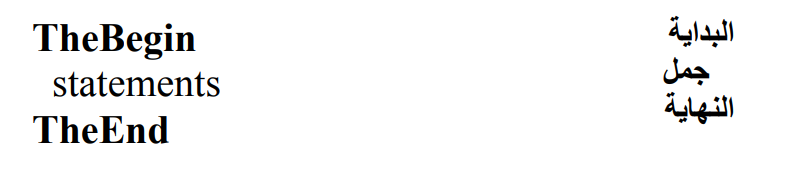
\includegraphics[width=10cm]{ch2-images/ARABLAN3.png}
\caption{ARABLAN Program \cite{al2007evaluation}}
\label{fig:ARABLAN Program}
\end{figure}

\begin{figure}[H]
\centering
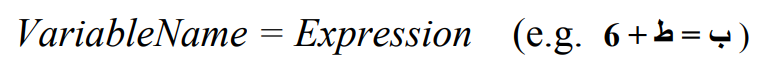
\includegraphics[width=10cm]{ch2-images/ARABLAN4.png}
\caption{ARABLAN Assignment Statement \cite{al2007evaluation}}
\label{fig:ARABLAN Assignment Statement}
\end{figure}

\begin{figure}[H]
\centering
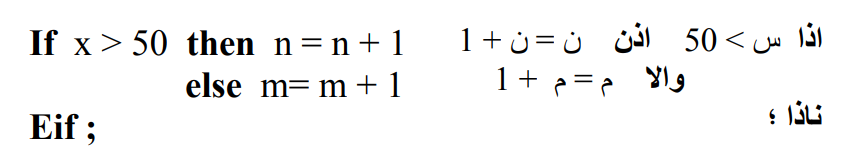
\includegraphics[width=10cm]{ch2-images/ARABLAN5.png}
\caption{ARABLAN Selection Statement \cite{al2007evaluation}}
\label{fig:ARABLAN Selection Statement}
\end{figure}

\begin{figure}[H]
\centering
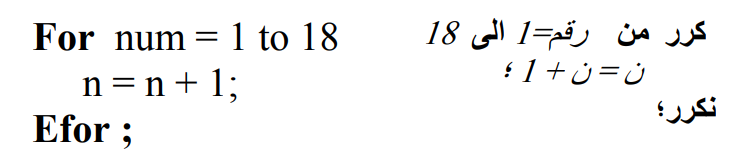
\includegraphics[width=10cm]{ch2-images/ARABLAN6.png}
\caption{ARABLAN Repetition Statement (For loop) \cite{al2007evaluation}}
\label{fig:ARABLAN Repetition Statement (For loop)}
\end{figure}

\begin{figure}[H]
\centering
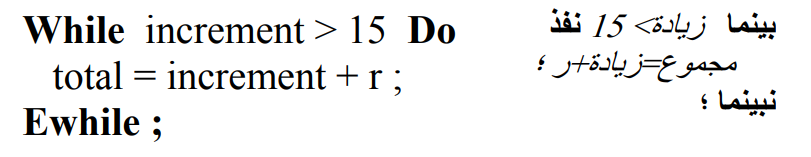
\includegraphics[width=10cm]{ch2-images/ARABLAN7.png}
\caption{ARABLAN Repetition Statement (While loop) \cite{al2007evaluation}}
\label{fig:ARABLAN Repetition Statement (while loop)}
\end{figure}

\begin{figure}[H]
\centering
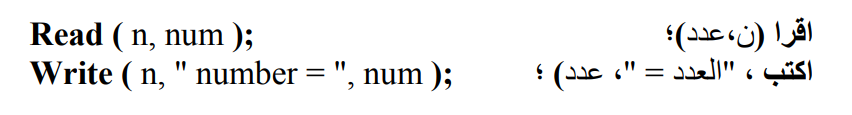
\includegraphics[width=10cm]{ch2-images/ARABLAN8.png}
\caption{ARABLAN Input/Output Statement \cite{al2007evaluation}}
\label{fig:ARABLAN Input/Output Statement}
\end{figure}

Finally, the last figure represents an example illustrating the structure of a subprogram in ARABLAN:

\begin{figure}[H]
\centering
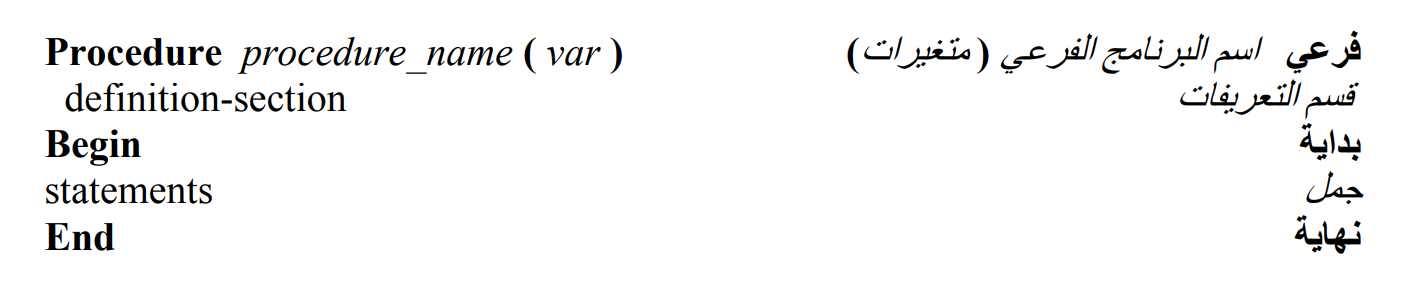
\includegraphics[width=15cm]{ch2-images/ARABLAN9.png}
\caption{ARABLAN Subprograms \cite{al2007evaluation}}
\label{fig:ARABLAN Subprograms}
\end{figure}

ARABLAN was put to the test in Bahrain schools to find out how well it taught Arab children computer programming. These studies and assessments aimed to establish whether ARABLAN was simple or challenging for pupils to learn. Additionally, homework assignments and data on students' language use were given to the students, and several language keywords were modified as a result of the statistics. For instance, the majority of pupils preferred using \<الثوابت> rather than \<ثوابت>. Consequently, this keyword was one of those that was altered in the language's syntax. Surveys were conducted to find out whether students prefer programming in their own language or in another language. The results showed that the majority of students preferred using Arabic. 

Results demonstrated that ARABLAN is clearly a step in the right direction for the future of Arabic programming languages. Numerous other elements of Arabic programming, such as the selection of terminology and mnemonics, the starting level, and so forth, need further study. Dr. Hamid tragically passed away suddenly just before finishing the study that he and Dr. Mansoor Al-A'ali had begun \cite{al2007evaluation}.
\subsection{DHAD}
Ben Othman \cite{othman2016arabic} created DHAD, which is another Arabic programming language. It aims to help non-English speaking students learn computer programming. DHAD is constructed in stages and has a number of parts. DHAD contains a compiler that converts source code into machine, C, and Assembly languages. A very useful editor is also available for writing programs using DHAD. Learning DHAD became an easy process because there is an interactive user interface that guides the user in learning DHAD through different complexity levels. The Exams component is one of the special components in DHAD’s architecture because it can be used by the instructor to create exams for their students. Here is a figure that shows the DHAD's architecture:
\begin{figure}[H]
\centering
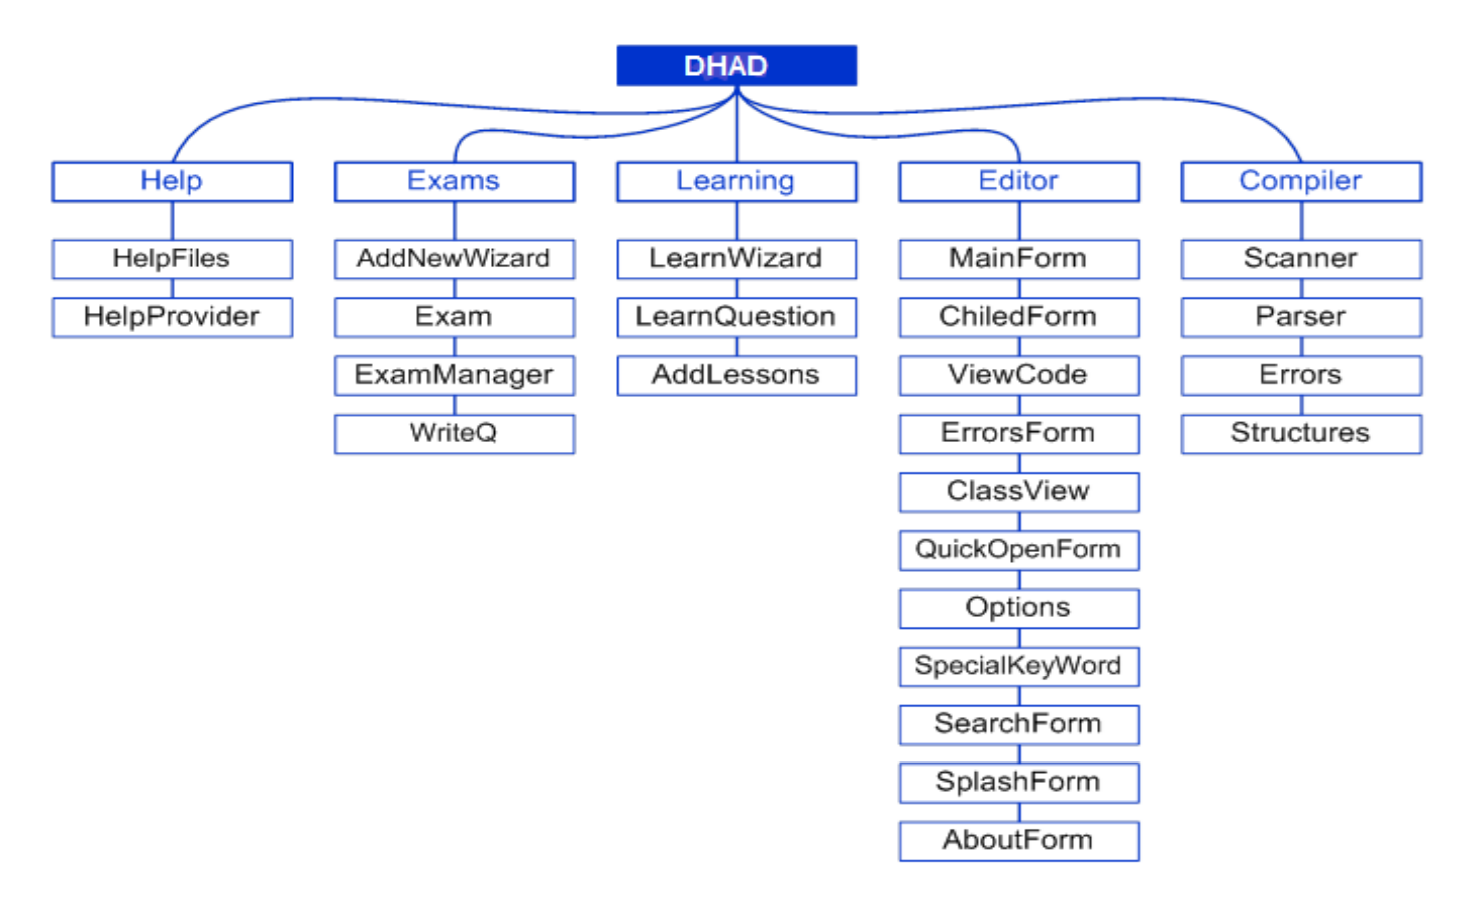
\includegraphics[width=8cm]{ch2-images/DHAD.png}
\caption{DHAD Tool’s Architecture \cite{othman2016arabic}}
\label{fig:DHAD Tool’s Architecture}
\end{figure}

A language's grammar must be decided before the compiler is created. The grammar is a combination of numerous high-level programming languages, including C, C++, and Pascal. It is the responsibility of the compiler to accept a file with the ".apl" extension (which stands for Arabic Programming Language) as input and construct the output files ``filename.c" and ``filename.asm" which contain translations of the written programs into C and Assembly, respectively. Depending on the compiler choices, different results are produced. The following figure explains the compiler's structure:

\begin{figure}[H]
\centering
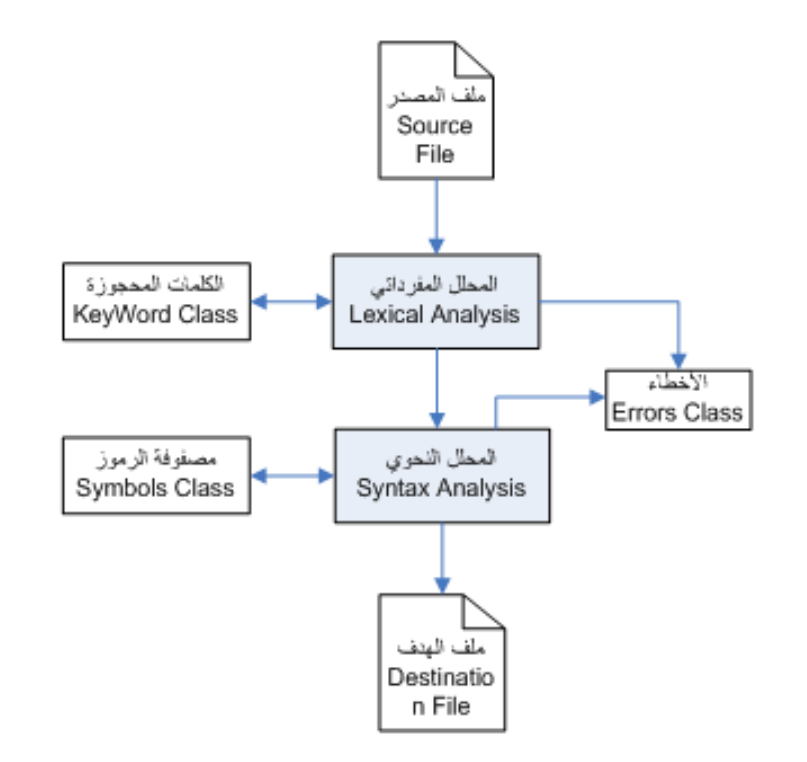
\includegraphics[width=8cm]{ch2-images/DHAD2.png}
\caption{DHAD Compiler's Structure \cite{othman2016arabic}}
\label{fig:DHAD Compiler's Structure}
\end{figure}

The syntax of DHAD is taken from three different languages which are C, C++, and Pascal, and modified to be easily used and understood by students later on. The following table gives some default keywords chosen for the DHAD programming language:

\begin{figure}[ht]
\centering
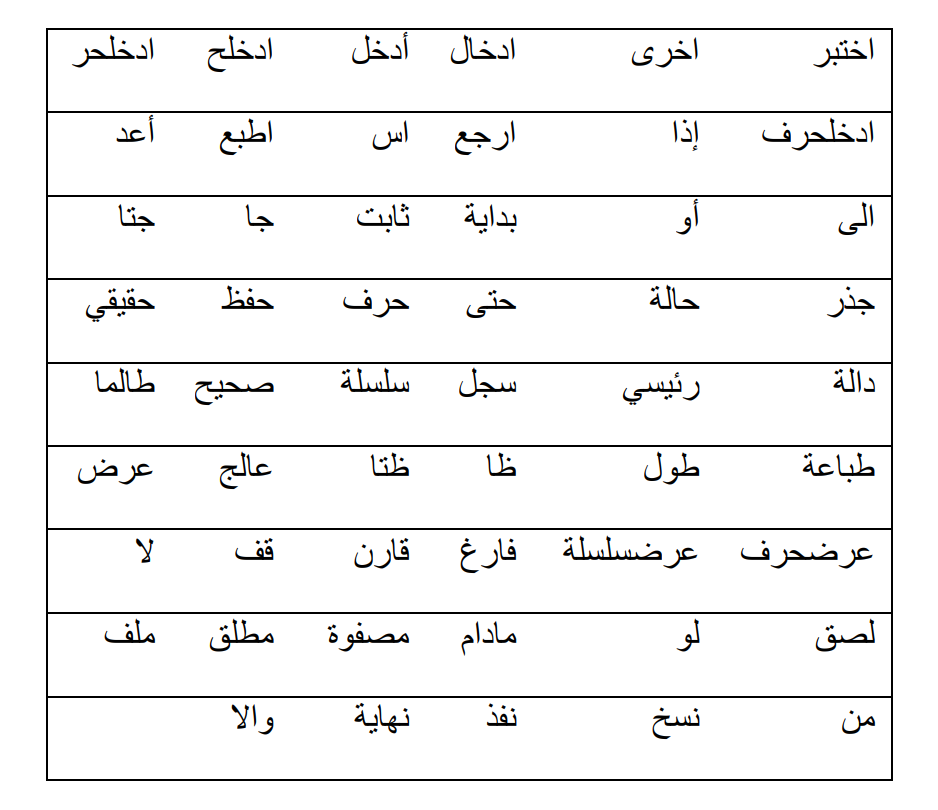
\includegraphics[width=10cm]{ch2-images/DHAD3.png}
\caption{DHAD Language Keywords \cite{othman2016arabic}}
\label{fig:DHAD Language Keywords}
\end{figure}

Multiple modules make up the compiler for DHAD. Prior to sending the tokens to the parser, the lexer must first read the program as a stream of characters and create tokens. The parser, which was developed according to the grammar of the language, determines whether the tokens sent by the lexer adhere to the grammar rules. The third module is then called by the parser, and if there are no syntax mistakes, it converts the source code to the target language.

The editor that supports the DHAD programming language has a help menu containing instructions' syntaxes with examples, a file menu for file management, and a compile menu with options for translation to C, Assembly language, and machine language. The program also allows users to customize keywords, giving them the ability to change any keyword in the language and revert back to the default keywords. 

Executing the program in the editor could be done in different ways. First, the direct execution in which the program is directly translated into machine language and then executed on the machine's processor. Another way is the cross-language translation in which the program is translated to Assembly or C according to the user's choice. DHAD has its own assembler that can be used separately, and then all messages like warnings, errors, and help are written in Arabic. Moreover, this assembler converts the translated Assembly code to machine language to be executed.

Future work on DHAD will concentrate mainly on how students could modify the code to have their own grammar rules for the compiler and their own control modules in the operating system.
\subsection{Alf..Eih}
Another Arabic programming language called Alf..Eih was created by Abdul Razaq et al \cite{razaq2019designing}. The decision to develop this language was contested. The usage of Arabic programming languages is impractical, according to opponents, who also said that any computer program should only be developed using English programming languages. On the other side, proponents asserted that there must be a programming language that fits the culture of the users. The following figure shows the general form of Alf..Eih:

\begin{figure}[H]
\centering
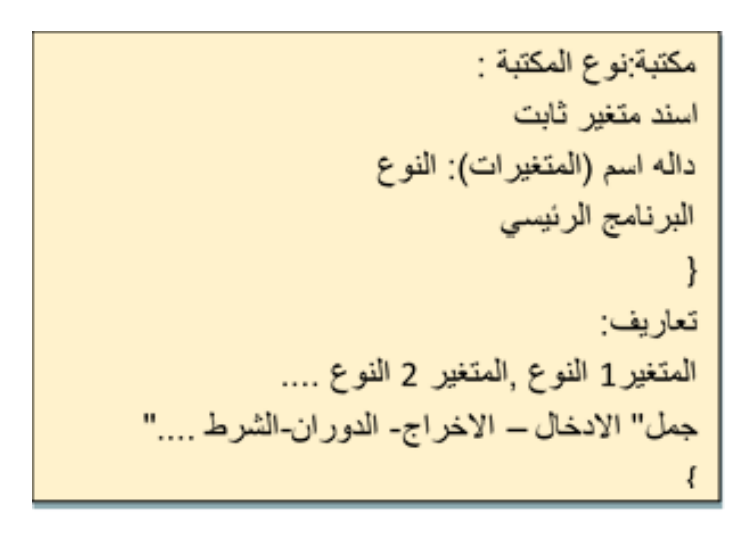
\includegraphics[width=10cm]{ch2-images/AlfEih.png}
\caption{Alf..Eih Program \cite{razaq2019designing}}
\label{fig:Alf..Eih Program}
\end{figure}

Alf..Eih is a localization of C++ programming language. This is done bearing in mind a non-expert user that can learn the language using simple ideas. The process of implementation involves a number of steps that will be discussed. The following figure shows an overview of the stages of implementation:

\begin{figure}[H]
\centering
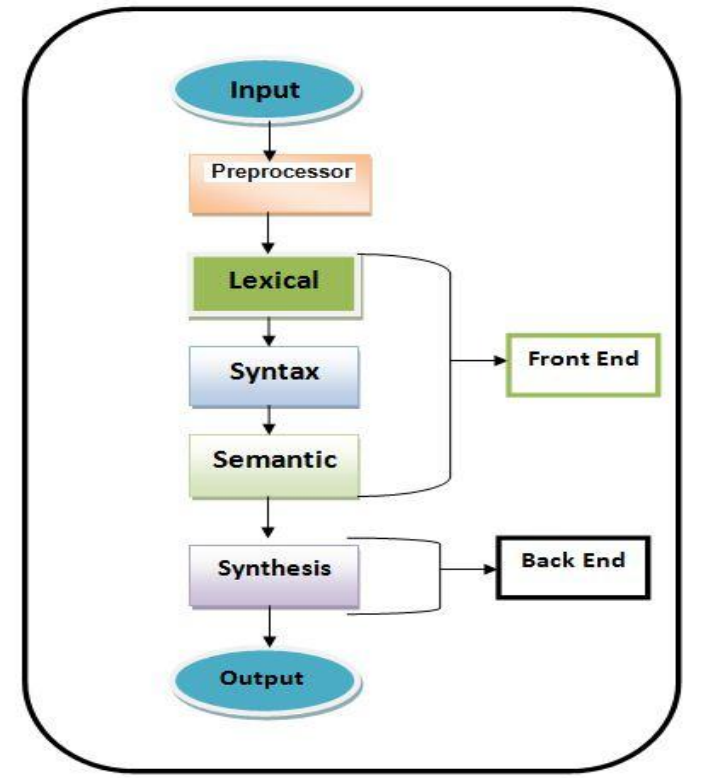
\includegraphics[width=5cm]{ch2-images/AlfEih2.png}
\caption{Alf..Eih stages of Implementation \cite{razaq2019designing}}
\label{fig:Alf..Eih stages of Implementation}
\end{figure}

The input program is first written in Arabic while adhering to the language's grammar rules. Spaces and newlines that cause issues are removed from the program after it has been written in the preprocessing step. The lexer examines the code after the preprocessing step to produce the tokens. If the component is absent, a lexical error takes place. The following stage, known as syntax, examines the input's grammatical structure to determine whether it is correct. Next comes the semantic stage, in which definitions are linked with the use and testing of each statement in terms of meaning. In the synthesis stage, the source code is translated to the equivalent C++ code, and after this stage, the code is ready to run. The following figures are examples illustrating each stage of the implementation:

\begin{figure}[H]
\centering
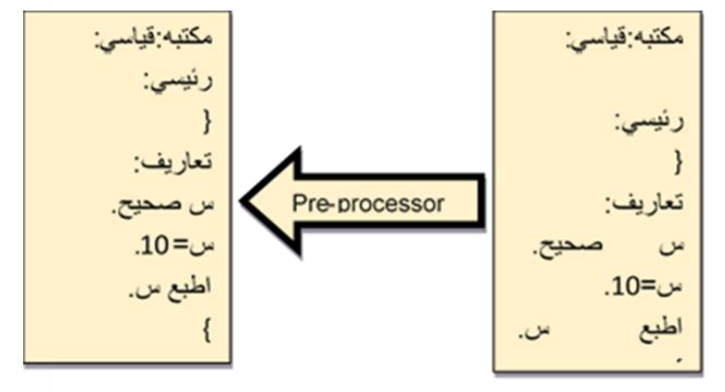
\includegraphics[width=7.5cm]{ch2-images/AlfEih3.png}
\caption{Alf..Eih Preprocessor \cite{razaq2019designing}}
\label{fig:Alf..Eih Preprocessor}
\end{figure}

\begin{figure}[H]
\centering
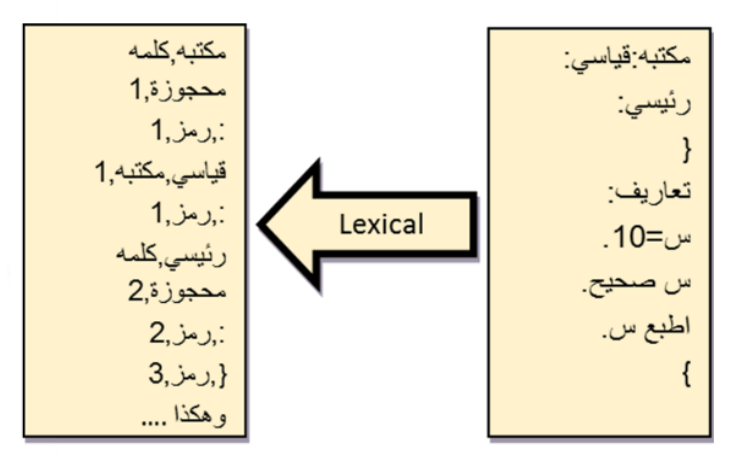
\includegraphics[width=7.5cm]{ch2-images/AlfEih4.png}
\caption{Alf..Eih Lexer \cite{razaq2019designing}}
\label{fig:Alf..Eih Lexer}
\end{figure}

\begin{figure}[H]
\centering
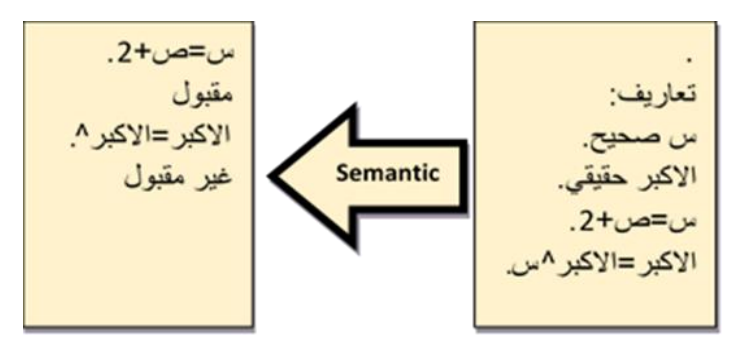
\includegraphics[width=7.5cm]{ch2-images/AlfEih5.png}
\caption{Alf..Eih Semantic \cite{razaq2019designing}}
\label{fig:Alf..Eih Semantic}
\end{figure}

\begin{figure}[H]
\centering
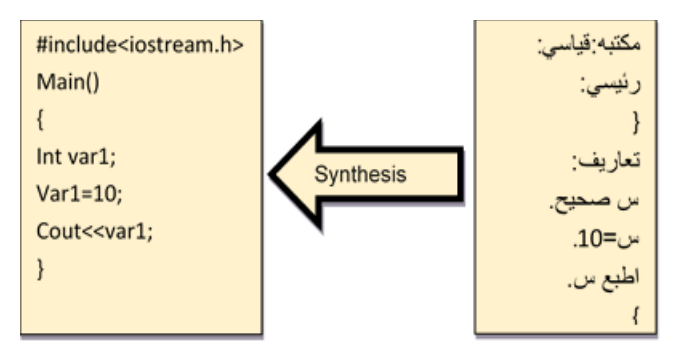
\includegraphics[width=7.5cm]{ch2-images/AlfEih6.png}
\caption{Alf..Eih Synthesis \cite{razaq2019designing}}
\label{fig:Alf..Eih Synthesis}
\end{figure}

It is recommended to put Alf..Eih in a test in schools to see its effectiveness in stimulating interest in computer programming. The language should also be expanded to include more library functions, loops, and classes ought to be added to the language. Students can better understand the ideas, guidelines, and needs of programming languages by adding Alf..Eih into the middle and high school curricula.
\subsection{Scratch}
 Dasgupta and Mako Hill \cite{dasgupta2017learning} created Scratch, a \ac{VPE}, whose primary goal is to help children learn to program. A unique source of observational data is provided by Scratch to answer questions about the effect of localization on learning due to its large user base and localization into dozens of languages. To specify the behavior of on-screen graphical objects known as sprites, programs in Scratch are created by dragging and dropping visual building blocks. In Scratch, blocks are the equivalent of tokens in text-based programming languages. They can be used in several ways, like moving a character on the screen, altering a variable, or repeating a series of instructions. The language preference is maintained between browser sessions through the use of \ac{HTTP} cookies. In the following figure, there is a Scratch code represented in four different languages:

\begin{figure}[ht]
\centering
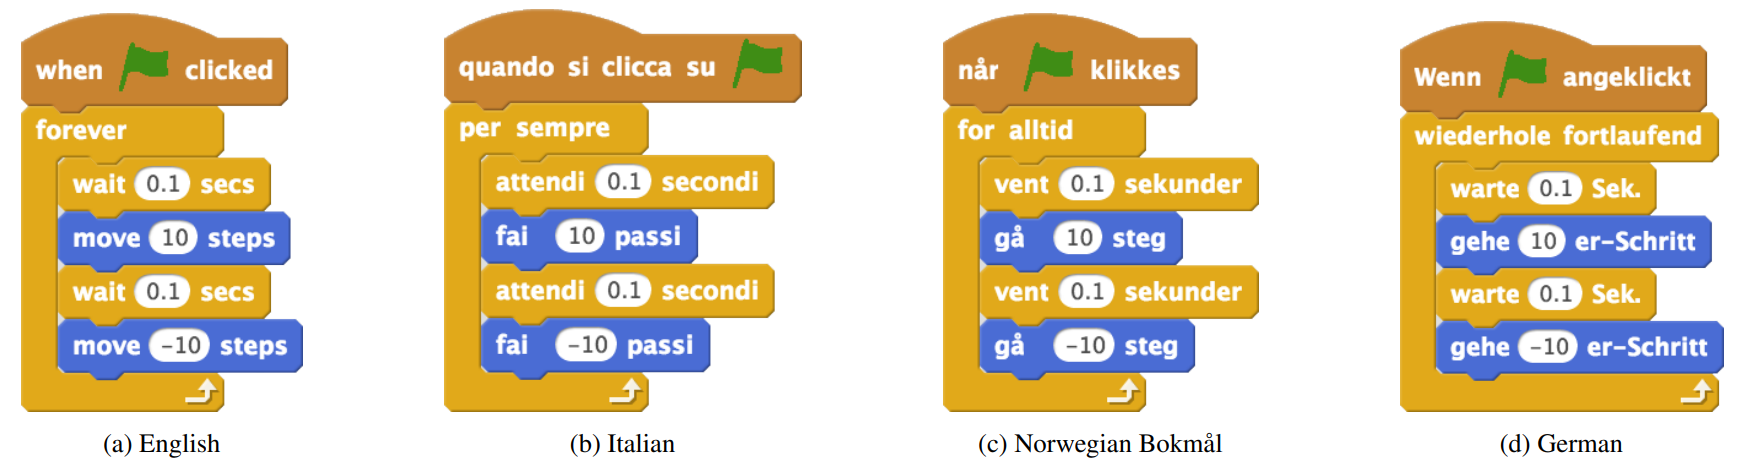
\includegraphics[width=15cm]{ch2-images/scratch.png}
\caption{Functionally Identical Scratch Code Represented in Four Different Languages \cite{dasgupta2017learning}}
\label{fig:Functionally Identical Scratch Code Represented in Four Different Languages}
\end{figure} 

Learning in Scratch is measured by the total number of blocks utilized, updated with each new project shared. This measure is used as the dependent variable in the analysis.

The study compares Italian-speaking users using Italian interfaces against those using non-localized English interfaces to determine whether people interact with Scratch using a localized interface. It is necessary to deduce each user's primary language and interface language to generate the variable using observation data. There are several reasons why someone would use Scratch in a language different than their native language. One reason is that the user could not be aware that the interface has a menu for changing languages or that there might be other technical issues.

Few languages are fully translated on Scratch because translation relies on volunteer work. Websites built with Scratch were updated frequently to correct bugs, so translations are now outdated. Because of this, the analysis will concentrate on the countries that volunteered the most in translation coverage. The authors use data on users' language preferences and primary languages to create a dummy variable indicating if a user's preferred interface language matches their home country's most widely used language. The study focuses on users from Portugal, Italy, Brazil, Germany, and Norway, and the authors conducted a similar analysis with two additional countries (France and Slovenia) as a double check. The following figure shows statistics for the usage of Scratch in different countries:

\begin{figure}[H]
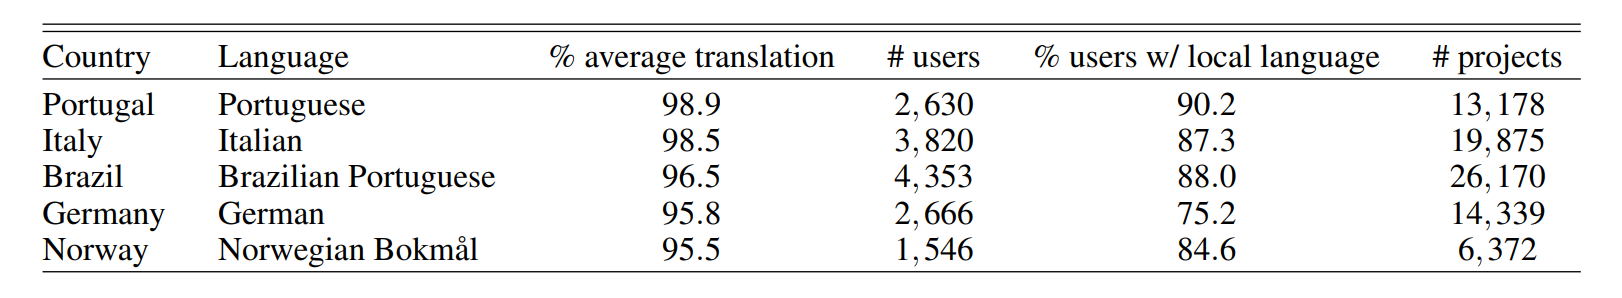
\includegraphics[width=15cm]{ch2-images/scratch2.png}
\caption{Countries included in the dataset used in this paper, along with the corresponding primary language, average translation level, number of users, proportion of users who use Scratch in the local language, and the total number of projects (with usable language data) per country \cite{dasgupta2017learning}}
\label{fig:Statistics for Usage of Scratch in Different Countries}
\end{figure} 

It is evident from the analysis and results that learners have better learning outcomes when using their language. The measurement of block repertoire has some drawbacks. One is that it can't tell whether a block is being used correctly or whether the user is aware of its purpose. To completely understand learners' comprehension, a qualitative study may be conducted.

Scratch is an excellent programming language because it offers a fully localized user interface, including programming language translations. The research supports the idea that young programmers learn faster with localized interfaces. Still, the most important effect of localization that the analysis fails to measure may be that working in the programmer's primary language encourages people who might not otherwise learn computer programming.
\subsection{Catrobat}
Awwad \cite{awwad2017localization} created Catrobat, a VPE similar to Scratch. The version of Catrobat, developed for Android smartphones, is named Catroid \cite{slany2012mobile} and is available on Google’s Play Store as ``Pocket Code”. It is a learning application that allows children and young people to create their own games, animations, and interactive apps on their phones or tablets using a VPE. Many countries promote programming education for primary and secondary school children, with VPEs typically used to teach programming. However, the release of VPEs worldwide requires the internationalization and localization of the product, particularly for bidirectional languages like Arabic, Persian, and Urdu. 

Many complex issues of bidirectional software localization remain unaddressed, preventing it from reaching its full potential. The Catrobat VPE has been localized into bidirectional and specifically to the Arabic language to address the difficulties that application developers confront. The localized VPE meets bidirectional requirements, complies with bidirectionality design guidelines, and can be used in programming education for young schoolchildren.

Internationalization and localization are crucial for software to be used in several locations. Internationalization refers to the process of re-engineering a system to support many languages and regions. In contrast, localization refers to the process of modifying an internationalized piece of software for use in a particular nation or culture by including locally relevant features and translated text. Due to its built-in support for localization components, an application that has been successfully internationalized is simpler to localize. Three key steps must be taken for localization to be successful: translating all text the user sees, adapting images and user interface components for diverse cultural contexts, and adding a locale to ensure that regional formats are presented correctly. The following figure shows the process of internationalization and localization:

\begin{figure}[H]
\centering
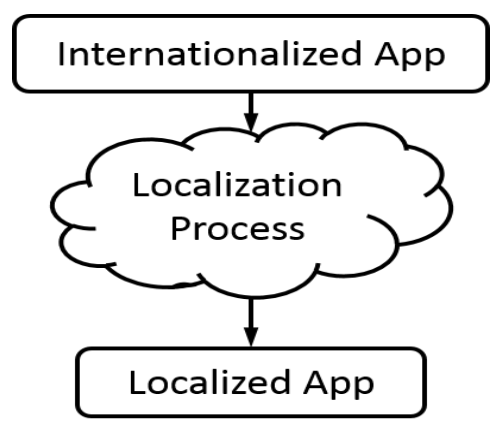
\includegraphics[width=7.5cm]{ch2-images/catrobat.png}
\caption{The Localization Process \cite{awwad2017localization}}
\label{fig:The Localization Process}
\end{figure} 

There were numerous difficulties encountered while attempting to localize Catrobat into bidirectional languages. However, solutions for establishing a dependable right-to-left user interface were offered. Arabic text and other complex scripts require unique rendering due to various script characteristics such as bidirectional text, contextual shaping, character reordering, and linking. Pocket Code has trouble with complex scripts, even if it can show many European languages. A program that displays text on the program's stage was developed to address this problem. Complex scripts cannot, however, be displayed using the bitmap font technology used by Pocket Code. The characters must first be saved in a buffer and then presented as a group for a bidirectional text to be rendered correctly. The bitmap image containing the text must be converted into a texture object to support complex bitmap font rendering for scripts such as Arabic, Urdu, and Persian. When the smartphone is set to Arabic, Pocket Code correctly displays the text with the proper directionality. The following figure shows a screenshot for the set and shows variable bricks with English and Arabic strings:

\begin{figure}[H]
\centering
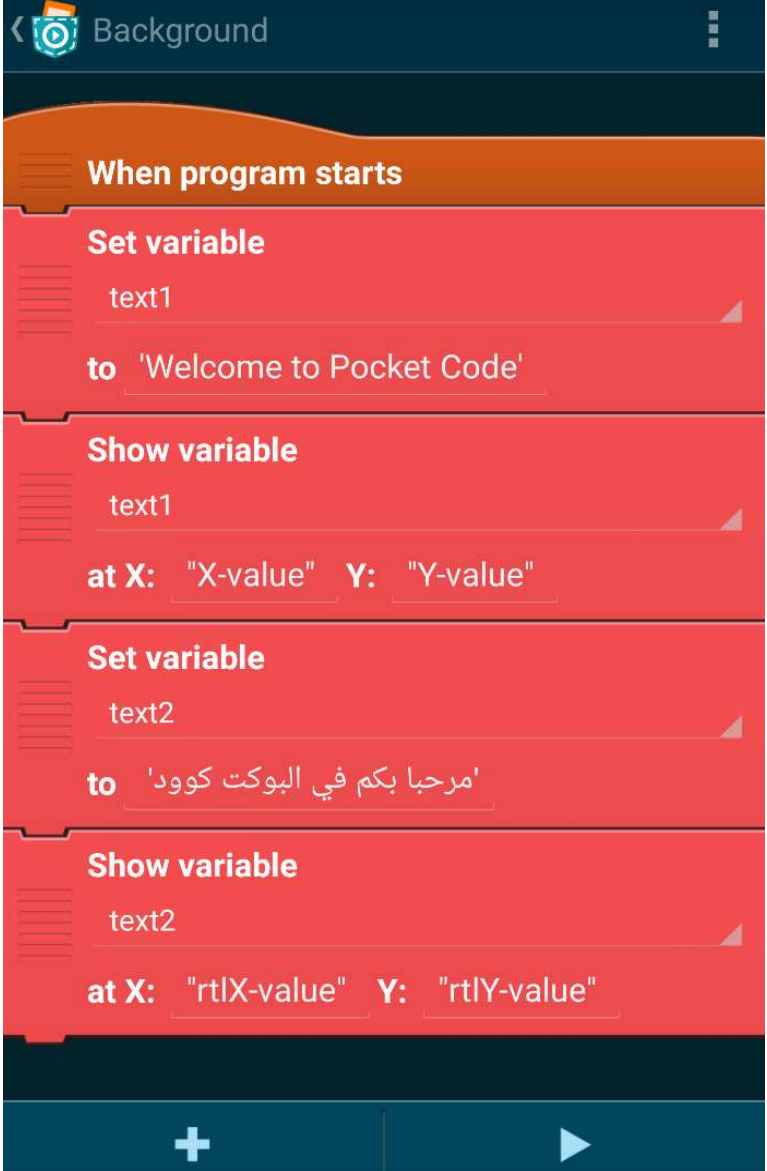
\includegraphics[width=7.5cm]{ch2-images/catrobat2.png}
\caption{Screenshot for the set and show variable bricks with English and Arabic strings \cite{awwad2017localization}}
\label{fig:Screenshot for the set and show variable bricks with English and Arabic strings}
\end{figure} 

Many challenges were faced in localizing a VPE for smartphones into bidirectional languages, specifically Arabic. The localization process involves adapting the software to suit the new culture and changing the source code and icons. The localization testing showed that Catrobat met bidirectional requirements that comply with bidirectionality design guidelines. 
\section{Summary}
To sum up, programming paradigms are one of the main aspects that must be considered while designing a programming language. To design a programming language, several tools are required to create the language: the lexer, parser, static analyzer, code optimizer, and code generator. Eclipse is one of the famous IDEs for writing and editing source code, especially for Java. Many attempts were made to design a localized programming language. Phoenix, ARABLAN, DHAD, and Alf..Eih were attempts made to create an Arabic programming language. Phoenix was the localized version of C\#, ARABLAN was the localized version of Pascal, DHAD was converted to machine code, C, assembly, while Alf..Eih was the localized version of C++. Moreover, Babylscript was a multilingual version of JavaScript, enabling users to write programmers in different languages. Finally, Scratch and Catrobat were VPEs created mainly for children to help them learn to program. 
